\chapter{From neurons to neural networks}
\label{ch:neural-networks}

\begin{learningobjectives}
After this chapter, you should be able to:
\begin{itemize}
  \item express a network first as connected neurons and then as matrix maps;
  \item distinguish preactivations $z^\ell$ from postactivations $a^\ell$;
  \item derive output and hidden errors by following computational paths;
  \item implement and gradient-check a vectorized dense layer;
  \item compare sigmoid--MSE, sigmoid--cross-entropy, and modern logits-based
  output contracts; and
  \item explain what automatic differentiation automates and what remains a
  modeling or systems decision.
\end{itemize}
\end{learningobjectives}

\begin{chapterconnection}
Chapter~\ref{ch:learning-api} separated a standalone estimator from a
differentiable component. We now use those components to build a network. The
derivation begins with literal neurons because every matrix entry should retain
a visible meaning. Only after tracing values forward and sensitivities backward
do we compress the calculation into vectorized layers.
\end{chapterconnection}

\section{Networks are computational graphs of neurons}

A feedforward neural network is a directed acyclic computational graph. Input
values enter layer zero, hidden layers form intermediate representations, and
an output layer produces quantities used by a loss or decision rule. For layer
$\ell$, let
\[
  w_{j,k}^{\ell}
\]
denote the weight from neuron $k$ in layer $\ell-1$ to neuron $j$ in layer
$\ell$. Then
\[
  z_j^\ell
  =\sum_{k=1}^{d_{\ell-1}}w_{j,k}^\ell a_k^{\ell-1}+b_j^\ell,
  \qquad
  a_j^\ell=\phi^\ell(z_j^\ell),
\]
with $a^0=x$.

\begin{definitionbox}{preactivation and postactivation}
The preactivation $z_j^\ell$ is the affine input to neuron $j$ in layer
$\ell$. The postactivation $a_j^\ell$ is the result after applying
$\phi^\ell$. Keeping $z$ and $a$ distinct is essential because the backward
pass needs $\phi'(z)$.
\end{definitionbox}

The bias $b_j^\ell$ is sometimes drawn as a fixed signal $1$ with a trainable
edge. This drawing is algebraically useful, but the bias is not an additional
measured feature.

\section{A concrete three--two--two network}

Consider three input signals, two hidden neurons, and two output neurons. The
first hidden neuron computes
\[
\begin{aligned}
z_1^1
  &=w_{1,1}^1x_1+w_{1,2}^1x_2+w_{1,3}^1x_3+b_1^1,\\
a_1^1&=\sigma(z_1^1).
\end{aligned}
\]
The second hidden neuron has its own weights and bias. The first output neuron
then computes
\[
  z_1^2=w_{1,1}^2a_1^1+w_{1,2}^2a_2^1+b_1^2,
  \qquad
  a_1^2=\sigma(z_1^2).
\]

This scalar view establishes three facts. A neuron receives postactivations
from the previous layer; each edge has a unique sending and receiving index;
and the same hidden activation can influence several downstream outputs. The
last fact will cause downstream gradient contributions to add.

Collecting neuron quantities yields
\[
  z^\ell=W^\ell a^{\ell-1}+b^\ell,
  \qquad
  a^\ell=\phi^\ell(z^\ell).
\]
For the example,
\[
W^1\in\mathbb R^{2\times3},\quad
b^1,z^1,a^1\in\mathbb R^2,\quad
W^2\in\mathbb R^{2\times2},\quad
b^2,z^2,a^2\in\mathbb R^2.
\]
Matrix form evaluates the same neuron equations together. It is an
implementation improvement, not a different mathematical model.

\begin{figure}[htbp]
  \centering
  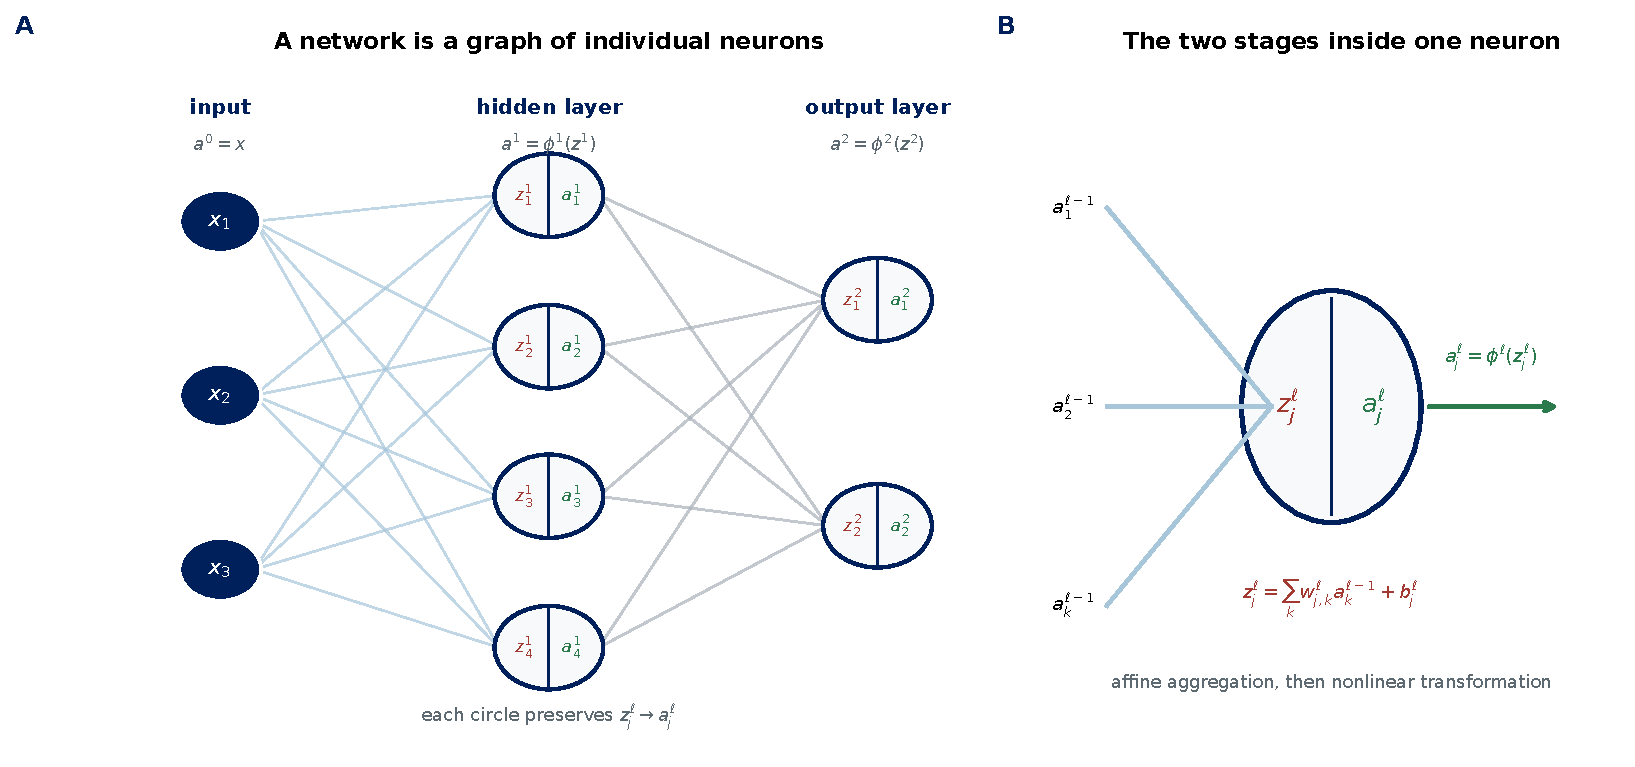
\includegraphics[width=\textwidth]{figures/generated/neural-network-anatomy.pdf}
  \caption{A layered network shown without hiding the individual neurons.
  Panel A distinguishes the affine preactivation $z_j^\ell$ from the
  postactivation $a_j^\ell$ at every hidden and output node. Panel B enlarges
  one neuron: incoming postactivations are aggregated affinely and then
  transformed. Matrix notation evaluates these same scalar operations in
  parallel.}
  \label{fig:neural-network-anatomy}
\end{figure}

\conceptcheck{Write $z_2^2$ without matrix notation. Identify the sender and
receiver represented by each subscript in $w_{2,1}^2$.}

\section{Why use a neural network?}

A single identity neuron represents an affine response surface. A single
sigmoid neuron represents a probability whose log-odds are affine; its
constant-probability contours and threshold decision boundary are hyperplanes.
These models are valuable precisely because this structure is restrictive and
interpretable. They cannot, without manually constructed features, express
several separated response regimes, an XOR interaction, or a hierarchy in
which small patterns combine into larger ones.

A neural network learns intermediate features together with the final
predictor. Width allows several neurons to detect different directions or
regimes and lets the next layer combine them. Depth allows later layers to
reuse and compose earlier features. The case for a network is therefore a
modeling hypothesis:
\begin{quote}
the response may be simpler as a composition of learned representations than
as one function of the original measurements.
\end{quote}
This hypothesis is often natural for images, sound, language, dynamical
systems, and other structured high-dimensional data. It is not automatically
correct for every table, and neural networks do not replace linear models,
trees, kernels, or domain-designed structure.

\subsection{Linear depth adds no expressive power}

Suppose two successive layers use identity activations. Then
\[
\begin{aligned}
f(x)
&=W^2(W^1x+b^1)+b^2\\
&=(W^2W^1)x+(W^2b^1+b^2).
\end{aligned}
\]
The composition is one affine map. Adding more linear layers changes a
factorization of its matrix, not the class of represented functions.

\begin{proposition}
A finite composition of affine maps is affine.
\end{proposition}

\begin{proof}
The calculation above proves closure for two maps. If the composition of the
first $m$ maps is $Ax+c$, composing one more affine map gives
$W(Ax+c)+b=(WA)x+(Wc+b)$, which is affine. Induction completes the proof.
\end{proof}

Nonlinear activation prevents this collapse. Figure~\ref{fig:neural-composition}
makes three distinct mechanisms visible. Affine depth remains a line. Several
ReLU neurons provide hinge features whose weighted sum can contain several
bends. Repeatedly composing one ReLU-representable tent map produces more
linear regions at each depth:
\[
T(x)=2\operatorname{ReLU}(x)
-4\operatorname{ReLU}\left(x-\frac12\right)
+2\operatorname{ReLU}(x-1),
\qquad 0\leq x\leq1.
\]
The example does not claim that more regions always generalize better. It
shows concretely what nonlinear composition can represent that an affine stack
cannot.

\begin{figure}[htbp]
  \centering
  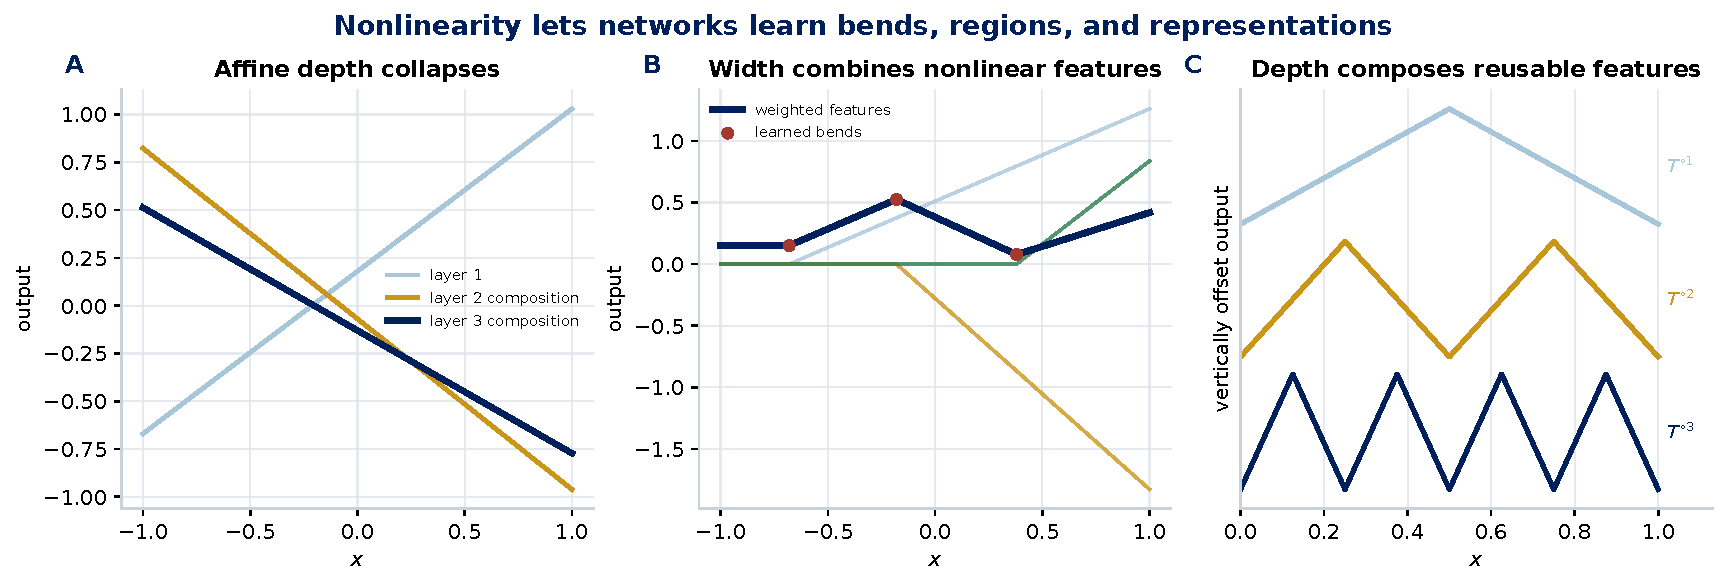
\includegraphics[width=\textwidth]{figures/generated/neural-composition-expressivity.pdf}
  \caption{Where expressive power enters. Panel A confirms that composing
  affine layers still produces one affine function. Panel B combines several
  ReLU hinge features to create a piecewise-linear function with multiple
  learned bends. Panel C composes the same tent feature: depth reuses an
  earlier computation and increases the number of linear regions. Expressive
  capacity is useful only when supported by data, regularization, and
  held-out evidence.}
  \label{fig:neural-composition}
\end{figure}

\subsection{Sigmoid and ReLU make different tradeoffs}

The sigmoid,
\[
  \sigma(z)=\frac1{1+\exp(-z)},
  \qquad
  \sigma'(z)=\sigma(z)(1-\sigma(z)),
\]
is smooth and historically useful for exposition. Its derivative becomes
small when $|z|$ is large, so saturated units transmit weak gradients.

The rectified linear unit
\[
  \operatorname{ReLU}(z)=\max(0,z)
\]
has derivative one for positive $z$ and zero for negative $z$, with a selected
subgradient convention at zero. ReLU often improves gradient propagation in
hidden layers, but a unit that remains negative for all relevant inputs can
become inactive. Other activations make other compromises; the appropriate
choice depends on output semantics, gradient flow, architecture, and evidence.

\section{A transparent first loss and its output error}

To preserve every chain-rule factor, begin with sigmoid at every neuron and
mean-squared error for a two-output, one-hot target,
\[
  C(W,B;x,y)=\frac12\sum_{r=1}^{2}(a_r^2-y_r)^2.
\]
Define the local error of neuron $j$ in layer $\ell$ by
\[
  \delta_j^\ell:=\frac{\partial C}{\partial z_j^\ell}.
\]
This definition matters. A delta is sensitivity with respect to a
\emph{preactivation}; it is not merely the observed prediction residual.

At the output,
\[
\begin{aligned}
\delta_j^2
&=\frac{\partial C}{\partial a_j^2}
  \frac{\partial a_j^2}{\partial z_j^2}\\
&=(a_j^2-y_j)\sigma'(z_j^2).
\end{aligned}
\]
Now follow one output weight $w_{j,k}^2$:
\[
\begin{aligned}
\frac{\partial C}{\partial w_{j,k}^2}
&=\frac{\partial C}{\partial a_j^2}
  \frac{\partial a_j^2}{\partial z_j^2}
  \frac{\partial z_j^2}{\partial w_{j,k}^2}\\
&=(a_j^2-y_j)\sigma'(z_j^2)a_k^1\\
&=\delta_j^2a_k^1.
\end{aligned}
\]
Because $\partial z_j^2/\partial b_j^2=1$,
\[
  \frac{\partial C}{\partial b_j^2}=\delta_j^2.
\]

\section{Hidden errors collect all downstream paths}

A hidden activation $a_j^1$ affects both output neurons. Its derivative must
therefore include both paths:
\[
\begin{aligned}
\delta_j^1
&=\frac{\partial C}{\partial z_j^1}\\
&=\left(
 w_{1,j}^2\delta_1^2+
 w_{2,j}^2\delta_2^2
\right)\sigma'(z_j^1).
\end{aligned}
\]
For a general layer,
\[
  \boxed{
  \delta^\ell
  =
  \left((W^{\ell+1})^\top\delta^{\ell+1}\right)
  \odot\phi^{\ell\prime}(z^\ell)
  }.
\]
The transpose reverses the forward connectivity: $W^{\ell+1}$ maps layer
$\ell$ activations forward, while $(W^{\ell+1})^\top$ collects sensitivities
from receiving neurons back to sending neurons. The Hadamard product
$\odot$ applies each neuron's local activation derivative.

Once $\delta^\ell$ is known,
\[
  \boxed{
  \frac{\partial C}{\partial W^\ell}
  =\delta^\ell(a^{\ell-1})^\top,
  \qquad
  \frac{\partial C}{\partial b^\ell}=\delta^\ell
  }.
\]

\begin{definitionbox}{backpropagation}
Backpropagation is an efficient organization of the chain rule on a layered
computational graph. It stores forward intermediates, initializes sensitivity
at the scalar loss, and reuses downstream derivatives while traversing the
graph in reverse.
\end{definitionbox}

\begin{misconceptionbox}
\textbf{Misconception:} backpropagation is the parameter-update algorithm.
\textbf{Correction:} backpropagation calculates derivatives. Gradient descent,
momentum, Adam, and other optimizers decide how those derivatives change
parameters.
\end{misconceptionbox}

\section{Batch vectorization}

Let $A^{\ell-1}\in\mathbb R^{n\times d_{\ell-1}}$ store observations by rows
and let $W^\ell\in\mathbb R^{d_\ell\times d_{\ell-1}}$. Then
\[
  Z^\ell=A^{\ell-1}(W^\ell)^\top+\mathbf1(b^\ell)^\top,
  \qquad
  A^\ell=\phi^\ell(Z^\ell).
\]
If $\Delta^\ell$ contains one delta row per observation, summing a mean loss
gives
\[
  \nabla_{W^\ell}C=(\Delta^\ell)^\top A^{\ell-1},
  \qquad
  \nabla_{b^\ell}C=(\Delta^\ell)^\top\mathbf1.
\]
The implementation must state whether its loss sums or averages across the
batch. A missing factor $1/n$ silently changes the effective learning rate.

A dense layer's forward operation retains its input and preactivation. Its
backward operation receives $\partial C/\partial A^\ell$, multiplies by
$\phi'(Z^\ell)$, forms parameter gradients, and returns
$\partial C/\partial A^{\ell-1}$. All layers compute gradients before an
optimizer updates any parameters; otherwise later derivatives would mix old
and new network states.

\section{Gradient checking a layer}

For parameter coordinate $\theta_j$, compare the analytical derivative with
\[
  g_j^{\mathrm{FD}}
  =
  \frac{C(\theta+he_j)-C(\theta-he_j)}{2h}.
\]
Use a tiny deterministic network in double precision, avoid sigmoid saturation
and ReLU kinks, restore each perturbed parameter, and compare with combined
absolute and relative tolerances.

Layer-level checks localize failures better than checking an entire large
network. Useful tests separately cover weight gradients, bias gradients, and
input gradients. Shape and call-order tests should verify that backward before
forward fails clearly.

\begin{warningbox}
A passing gradient check establishes agreement between two calculations near
one test point. It does not prove that the loss matches the scientific question,
that data splitting is valid, or that optimization will generalize.
\end{warningbox}

\section{Output losses change the initial backward signal}

The transparent sigmoid--MSE example yields
\[
  \delta^L=(a^L-y)\odot\sigma'(z^L).
\]
For a binary sigmoid output paired with cross-entropy, the activation and loss
derivatives cancel:
\[
  \delta^L=a^L-y.
\]
Thus the simplified residual is correct for the canonical logistic objective
but not for sigmoid paired with mean-squared error.

For $K$ mutually exclusive classes, a modern implementation commonly emits
logits $z\in\mathbb R^K$ and combines softmax with cross-entropy:
\[
  p_k=\frac{\exp z_k}{\sum_r\exp z_r},
  \qquad
  \ell(z,y)=-\log p_y.
\]
Stable code shifts logits or uses a fused log-sum-exp operation. The gradient
with respect to logits is $p-e_y$. A fused loss both clarifies its input
contract and avoids taking logarithms of rounded probabilities.

The hidden-layer recursion remains the same. Changing the output loss changes
where reverse propagation begins; it does not replace backpropagation.

\section{Initialization and gradient flow}

If sigmoid preactivations begin with large magnitude, activations saturate and
gradients shrink. Initializing every parameter with unscaled standard normal
noise becomes increasingly hazardous as fan-in grows.

Xavier or Glorot scaling is motivated by preserving forward and backward
variance for approximately symmetric activations under explicit independence
assumptions. He scaling is commonly paired with ReLU-like activations. These
are starting principles rather than universal theorems about training.
Initialization, activation, normalization, depth, and optimizer interact.

Record architecture, initializer, random seed, dtype, data order, and
preprocessing. Inspect activation distributions, gradient norms, and
nonfinite values when training stalls. Random biases scaled like weights are
not automatically justified; zero or problem-informed bias initialization is
often clearer.

\section{A real-data training argument}

Consider image-derived measurements from breast-mass samples. A bounded manual
network can demonstrate the complete mechanism:
\begin{enumerate}
  \item preserve a stratified held-out test partition;
  \item fit scaling on training observations only;
  \item train a small hidden layer and two-output classifier;
  \item record the training objective;
  \item freeze parameters before final evaluation; and
  \item report a confusion matrix and task-relevant metrics.
\end{enumerate}

The training curve is optimization evidence. A held-out confusion matrix is
decision evidence. Neither establishes probability calibration, clinical
transportability, or acceptable harm. Two independent sigmoid outputs need
not sum to one, and MSE is retained in the first experiment to match the
derivation rather than because it is the strongest modern multiclass contract.

\begin{workedexample}{from transparent derivation to modern candidate}
A team first trains a $3$--$2$--$2$ sigmoid network on a four-observation logic
problem. It checks every dense-layer derivative by central differences. It then
trains a small network on versioned diagnostic measurements, keeping the test
partition untouched.

For the release candidate, the team changes hidden activations to ReLU and the
output to logits consumed by cross-entropy. It rechecks gradients, chooses a
checkpoint with validation data, and loads the saved artifact in a fresh
process. The model card reports class order, preprocessing identity, seed
variability, balanced accuracy, confusion counts, and known limits. The manual
network established mechanism; the framework implementation supplies scalable
machinery without weakening the evidence contract.
\end{workedexample}

\section{Automatic differentiation and framework boundaries}

Reverse-mode automatic differentiation records primitive tensor operations and
applies their local derivative rules backward from a scalar loss. A framework
also supplies optimized kernels, accelerators, modules, mini-batch data
loading, optimizers, and serialization.

It does not decide:
\begin{itemize}
  \item whether the target is a valid scientific construct;
  \item whether preprocessing leaks validation or future information;
  \item whether output and loss match the desired probability claim;
  \item whether a metric represents operational cost;
  \item whether errors concentrate in consequential groups; or
  \item whether inference reproduces training-time feature order and state.
\end{itemize}

\begin{professionalbox}
The manual network is a microscope, not a production framework. Use it to
derive and test the mechanism. Then use a mature tensor framework while
retaining explicit data, objective, evaluation, serialization, and monitoring
contracts.
\end{professionalbox}

Training and evaluation modes can differ because of dropout and batch
normalization. A released artifact includes parameters, architecture,
preprocessing reference, class order, checkpoint-selection evidence, software
versions, and inference mode. A fresh-process test should reload it and compare
predictions on versioned fixtures within declared tolerances.

\section{Exercises}
\begin{enumerate}
  \item Write every scalar equation in a $3$--$2$--$2$ sigmoid network and
  annotate its shape.
  \item Derive $\partial C/\partial w_{1,2}^1$ by listing both output paths
  before collecting them into matrix notation.
  \item Prove the softmax--cross-entropy logit gradient is $p-e_y$.
  \item Design finite-difference tests for a dense layer's weights, biases, and
  input gradient.
  \item Replace hidden sigmoid with ReLU. State the derivative convention at
  zero and justify an initializer.
  \item Explain why a decreasing training loss and high test accuracy still do
  not establish calibrated clinical probabilities.
  \item Specify a pull request that adds mini-batching or serialization to the
  course implementation. Include shape, randomness, failure, and regression
  tests.
\end{enumerate}

\begin{chapterreview}
A network connects individual affine neurons through nonlinear activations.
Preactivations $z^\ell$ and postactivations $a^\ell$ must remain distinct.
Backpropagation initializes an output sensitivity, sums every downstream path
into hidden deltas, and forms weight gradients from local errors and incoming
activations. Matrix operations vectorize the same neuron equations. Output
losses determine the first backward signal; activations and initialization
shape gradient flow. Automatic differentiation scales derivative calculation,
but scientific validity, evaluation, artifact integrity, and operational
judgment remain human responsibilities.
\end{chapterreview}

\begin{notebooklink}
Lecture 12 notebook 00 designs the reusable single-neuron and component
interfaces. Lecture 12 notebook 01 begins with literal neurons, derives
backpropagation path by path, gradient-checks a vectorized dense layer, and
evaluates a bounded manual network before crossing to automatic differentiation.
\end{notebooklink}
